\chapter{Meta}

\section{Hintergrund}

Das Internet der Dinge wird Tag für Tag größer. Der Einfluss den smarte Geräte in modernen Haushalten haben wird ständig erhöht. Die meisten Hersteller von smarten Geräten zielen auf Benutzerfreundlichkeit und Einfachkeit ab. Die vielen Do-It-Yourself Enthusiasten rücken für sie in den Hintergrund. Einer der wichtigsten und am häufigsten genutzten Mechanismen in einem Haushalt sind Schlösser.  Da nicht jeder, der selbst gerne Sachen in die Hand nimmt, die Fähigkeit oder Zeit besitzt, ein sicheres und smartes Türschloss von Grund auf zu entwerfen und aufzubauen, haben wir uns entschieden, ein intelligentes Türschloss zu entwickeln.

\section{Namensherkunft}

Der Name \textbf{Shulker} stammt ursprünglich aus dem Videospiel \textit{Minecraft}. Der Shulker ist eine Kreatur, die sich in einer Box verschanzt.

\begin{figure}[H]
    \begin{center}
        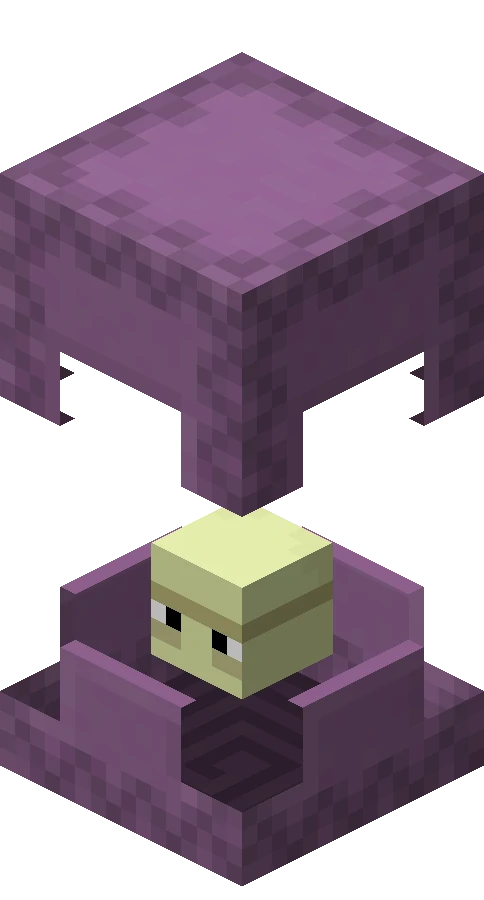
\includegraphics[width=0.22\textwidth]{images/Intro/Shulker.png}
        \caption{Die Kreatur \textbf{Shulker} aus dem Videospiel \textit{Minecraft}}
        \cite{mcwiki2015}
    \end{center}
\end{figure}

\newpage